\documentclass[tikz,border=2cm]{standalone}
\begin{document}
    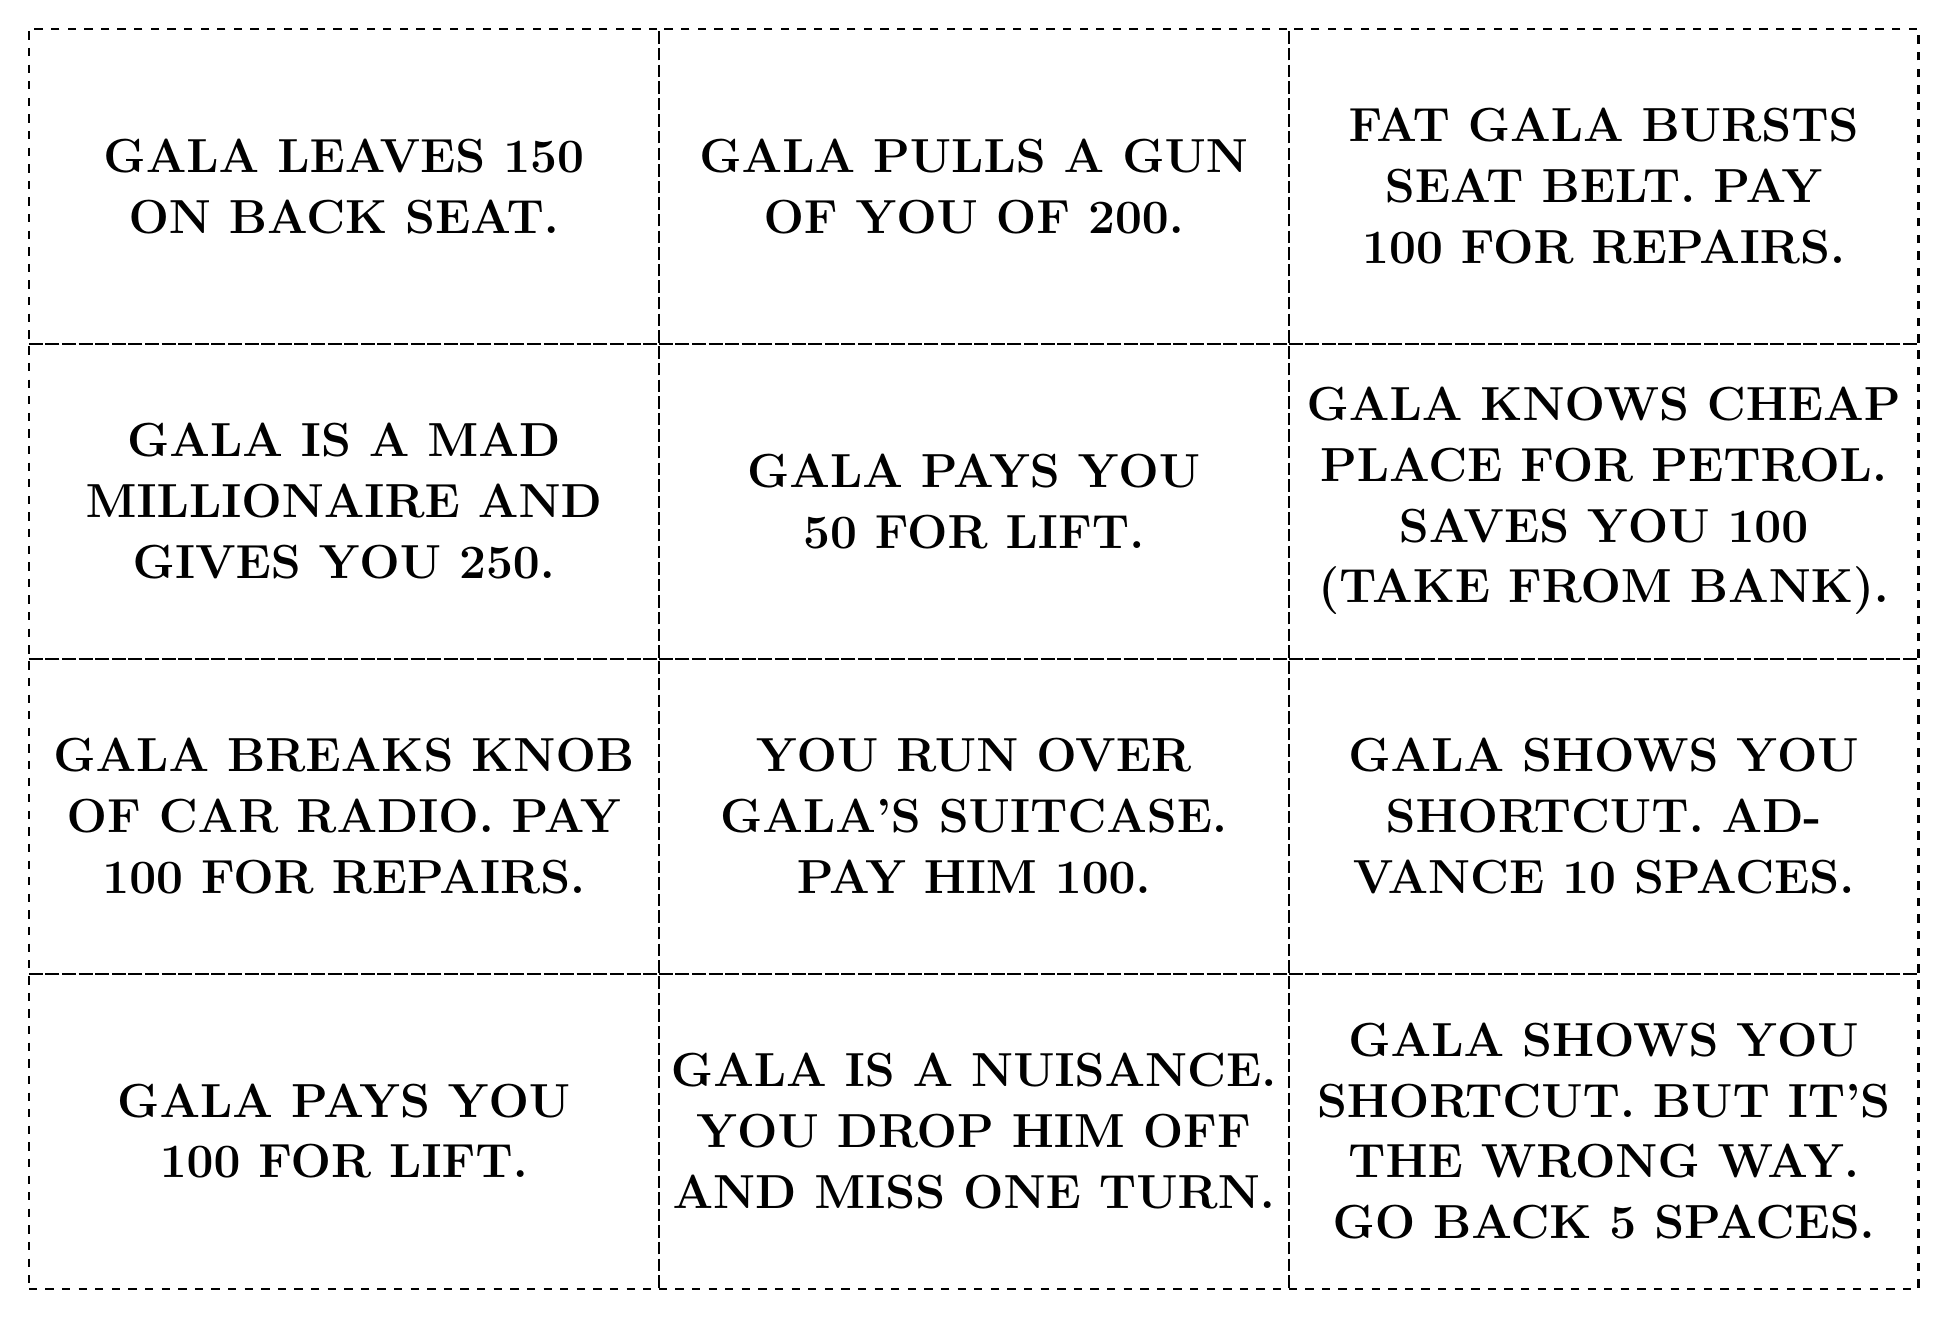
\begin{tikzpicture}
        [every node/.style={rectangle,draw,dashed,thick,inner sep=0pt,align=center},
        card/.style={minimum height=4cm,minimum width=8cm,text width=8cm,font=\LARGE\bfseries},
        ]
        \node[card] (card-1) at (0, 0) {GALA PAYS YOU 100 FOR LIFT.};
        \node[card] (card-2) at (8, 0) {GALA IS A NUISANCE. YOU DROP HIM OFF AND MISS ONE TURN.};
        \node[card] (card-3) at (16, 0) {GALA SHOWS YOU SHORTCUT. BUT IT'S THE WRONG WAY. GO BACK 5 SPACES.};
        \node[card] (card-4) at (0, 4) {GALA BREAKS KNOB OF CAR RADIO. PAY 100 FOR REPAIRS.};
        \node[card] (card-5) at (8, 4) {YOU RUN OVER GALA'S SUITCASE. PAY HIM 100.};
        \node[card] (card-6) at (16, 4) {GALA SHOWS YOU SHORTCUT. ADVANCE 10 SPACES.};
        \node[card] (card-7) at (0, 8) {GALA IS A MAD MILLIONAIRE AND GIVES YOU 250.};
        \node[card] (card-8) at (8, 8) {GALA PAYS YOU 50 FOR LIFT.};
        \node[card] (card-9) at (16, 8) {GALA KNOWS CHEAP PLACE FOR PETROL. SAVES YOU 100 (TAKE FROM BANK).};
        \node[card] (card-10) at (0, 12) {GALA LEAVES 150 ON BACK SEAT.};
        \node[card] (card-11) at (8, 12) {GALA PULLS A GUN OF YOU OF 200.};
        \node[card] (card-12) at (16, 12) {FAT GALA BURSTS SEAT BELT. PAY 100 FOR REPAIRS.};
    \end{tikzpicture}
\end{document}